\thispagestyle{fancy}
\vspace*{40 pt}
\subsection{Novo pedido página 1} \label{sec:telaNovoPedidoP1}
Essa tela é carrega quando o usuário clica no botão de novo pedido na tela de visualização de pedidos.
\vspace*{\fill}
\begin{figure}[h]
    \centering
    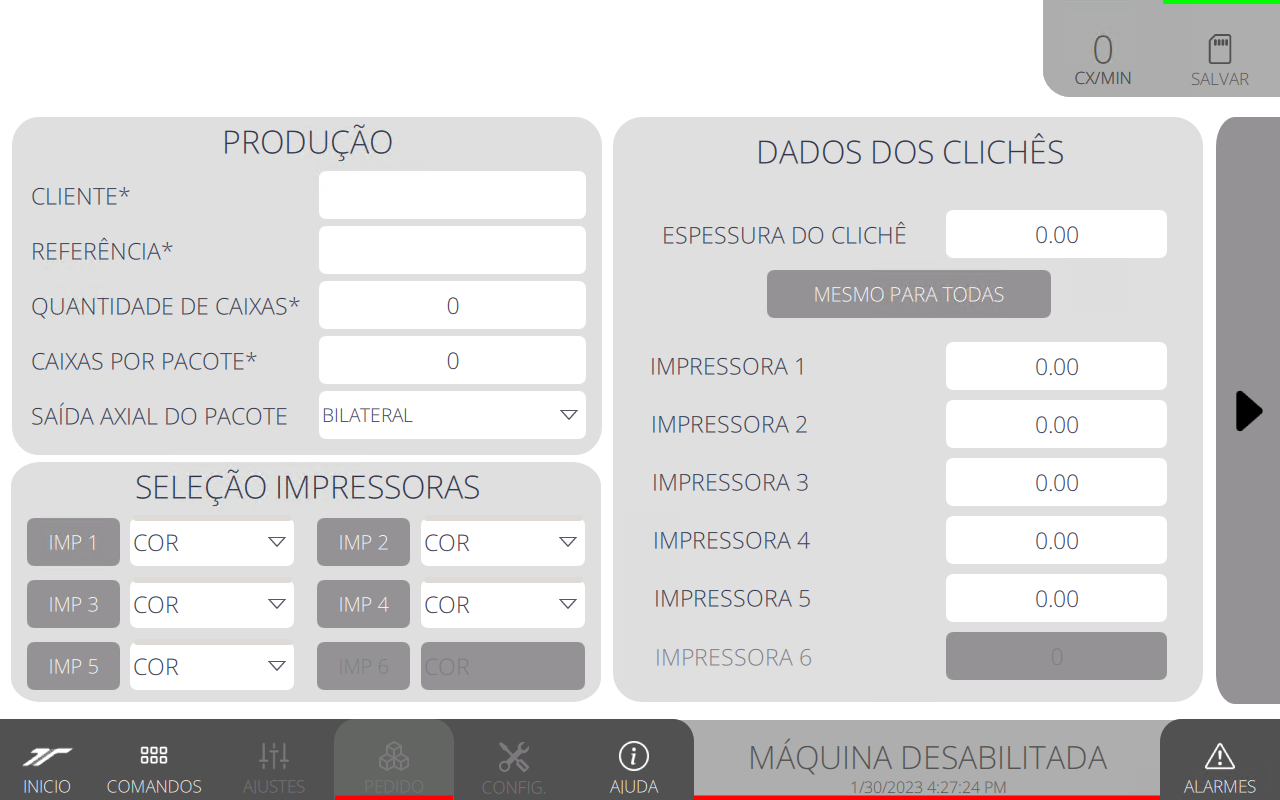
\includegraphics[width=480 px,height=300 px]{src/imagesICV/09-request/new/Tela-Principal.png}
\end{figure}
\vspace*{\fill}

\newpage
\thispagestyle{fancy}
\vspace*{40 pt}
\subsubsection{\small{Informações do pedido}} \label{sec:telaNovoPedidoP1InformacoesPedido}
\vspace*{\fill}
\begin{figure}[h]
    \centering
    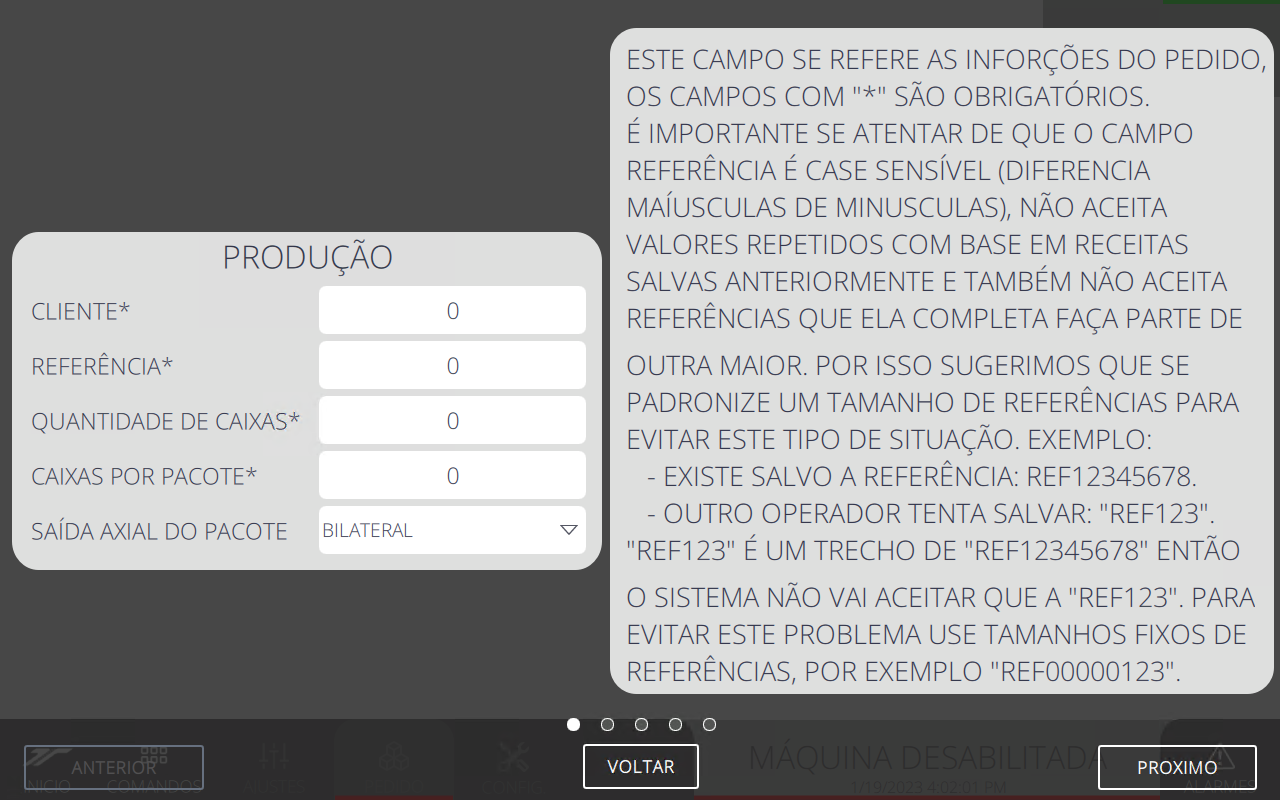
\includegraphics[width=576 px,height=360 px]{src/imagesICV/09-request/new/e-1-COM-ERRO-DIGITAÇÃO.png}
\end{figure}
\vspace*{\fill}

\newpage
\thispagestyle{fancy}
\vspace*{40 pt}
\subsubsection{\small{Seleção de impressora}} \label{sec:telaNovoPedidoP1SelecaoImpressora}
\vspace*{\fill}
\begin{figure}[h]
    \centering
    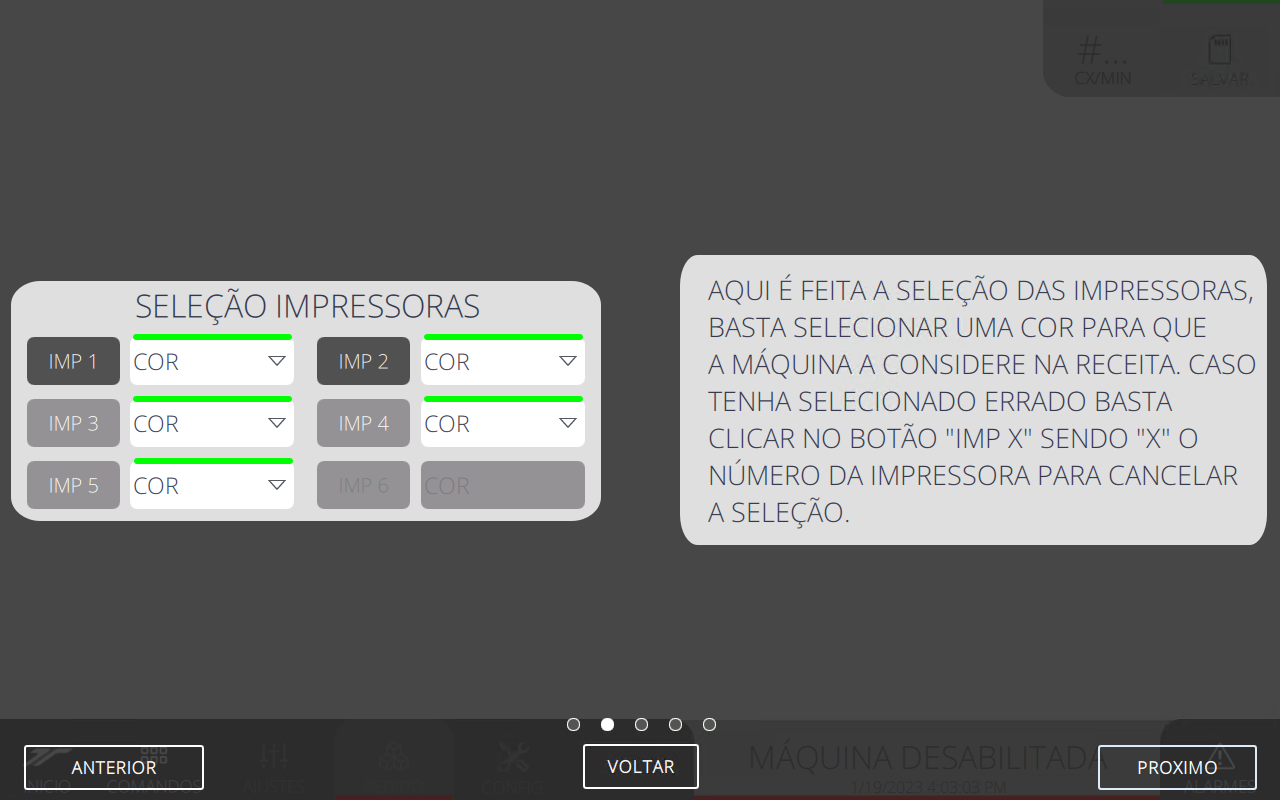
\includegraphics[width=576 px,height=360 px]{src/imagesICV/09-request/new/e-2.png}
\end{figure}
\vspace*{\fill}

\newpage
\thispagestyle{fancy}
\vspace*{40 pt}
\subsubsection{\small{Dados dos clichês}} \label{sec:telaNovoPedidoP1DadosCliche}
\vspace*{\fill}
\begin{figure}[h]
    \centering
    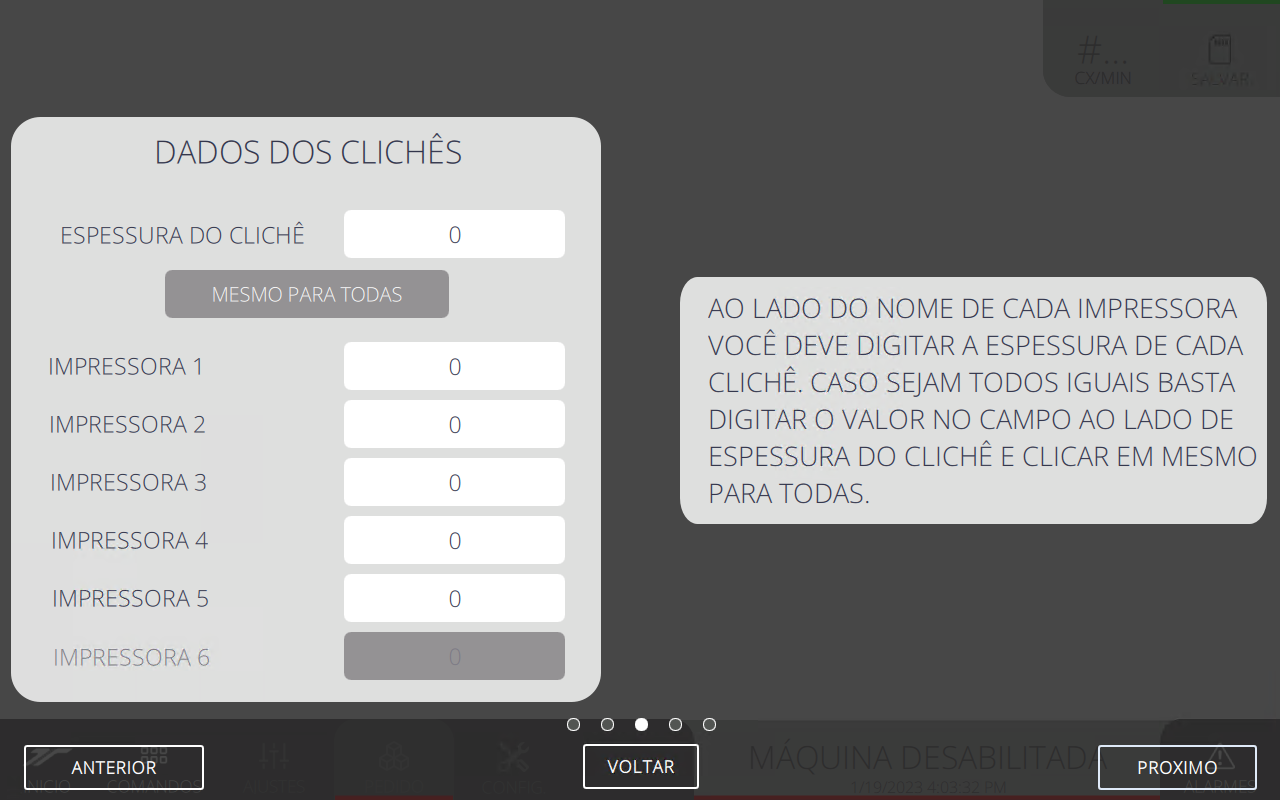
\includegraphics[width=576 px,height=360 px]{src/imagesICV/09-request/new/e-3.png}
\end{figure}
\vspace*{\fill}

\newpage
\thispagestyle{fancy}
\vspace*{40 pt}
\subsubsection{\small{Requisitos para liberar a próxima página}} \label{sec:telaNovoPedidoP1RequisitosLiberarProximaPagina}
\vspace*{\fill}
\begin{figure}[h]
    \centering
    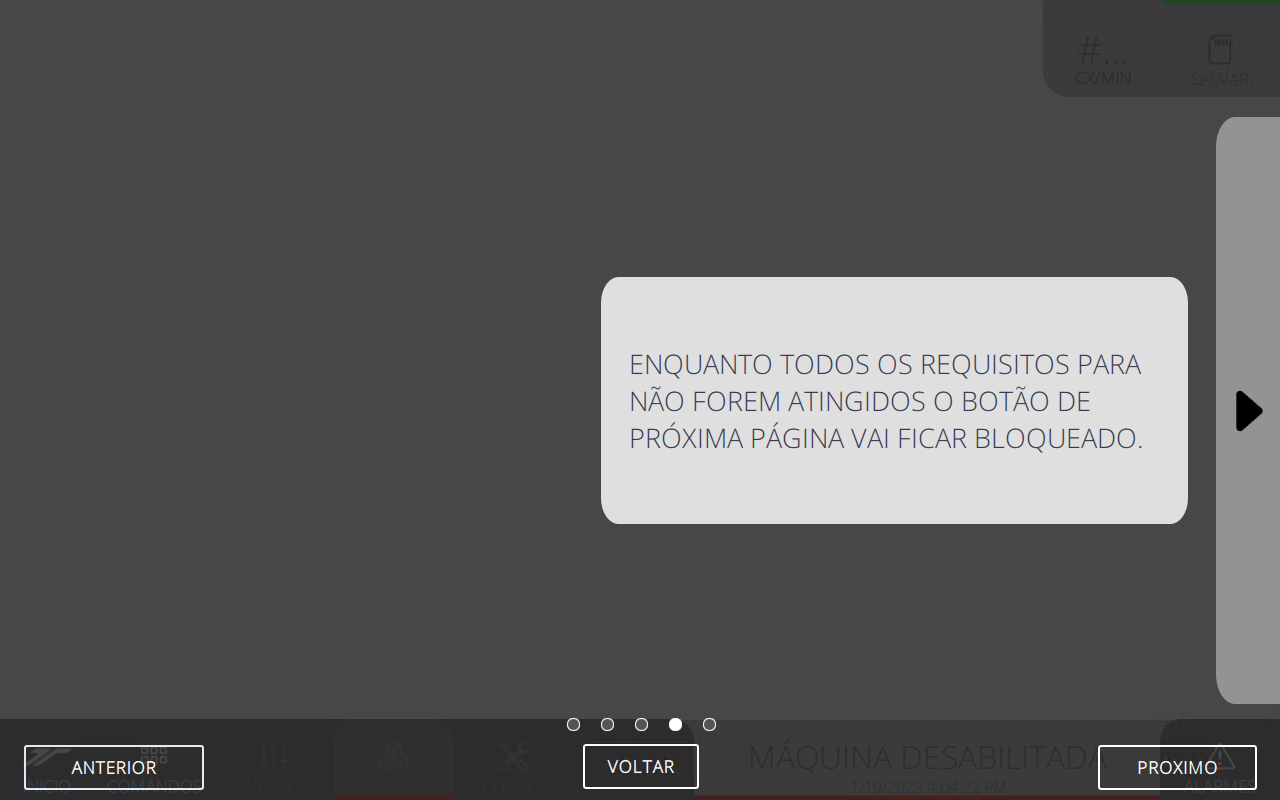
\includegraphics[width=576 px,height=360 px]{src/imagesICV/09-request/new/e-4-COM-ERRO-DIGITAÇÃO.png}
\end{figure}
\vspace*{\fill}

\newpage
\thispagestyle{fancy}
\vspace*{40 pt}
\subsubsection{\small{Botão próxima página liberada}} \label{sec:telaNovoPedidoP1BotaoProximaPaginaLiberada}
\vspace*{\fill}
\begin{figure}[h]
    \centering
    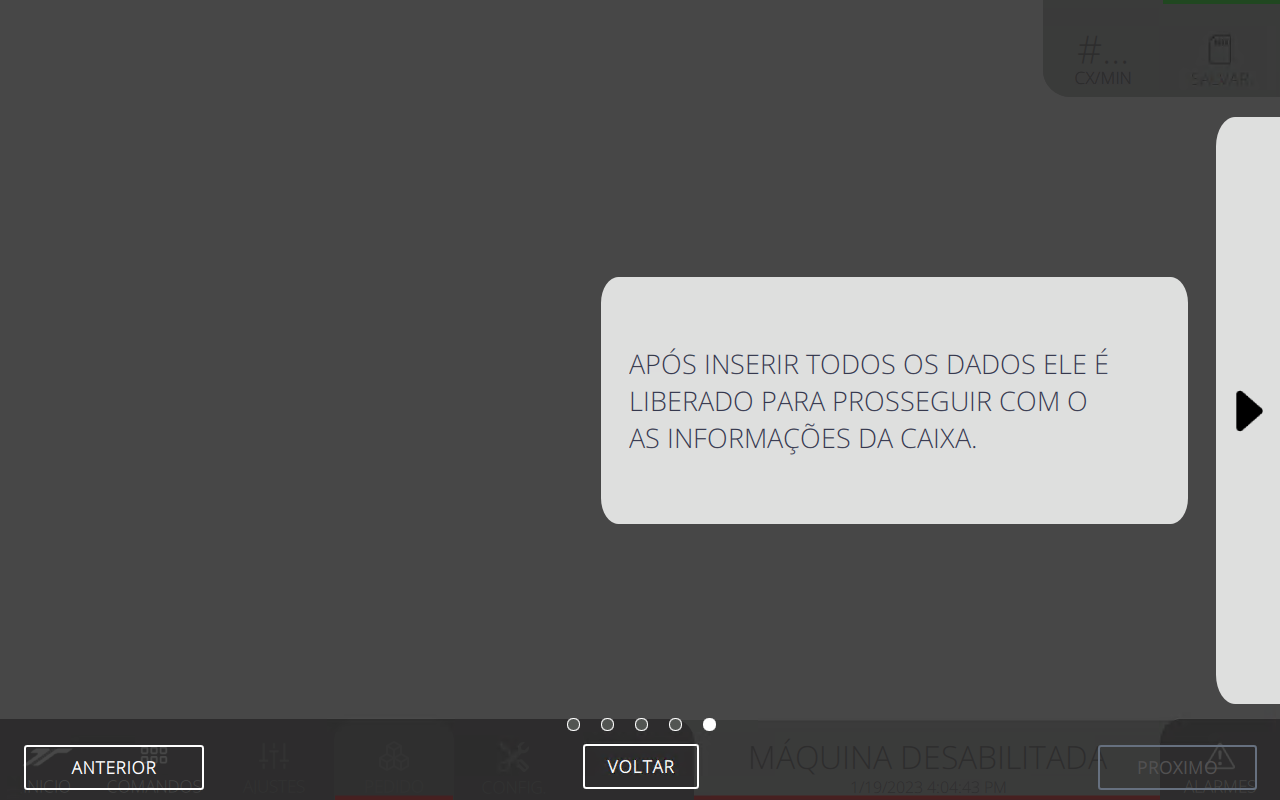
\includegraphics[width=576 px,height=360 px]{src/imagesICV/09-request/new/e-5.png}
\end{figure}
\vspace*{\fill}

\newpage
\thispagestyle{fancy}
\vspace*{40 pt}
\subsection{Novo pedido página 2} \label{sec:telaNovoPedidoP2}
Essa tela é carrega quando o usuário clica no botão de próxima página na tela de novo pedido página 1.
\vspace*{\fill}
\begin{figure}[h]
    \centering
    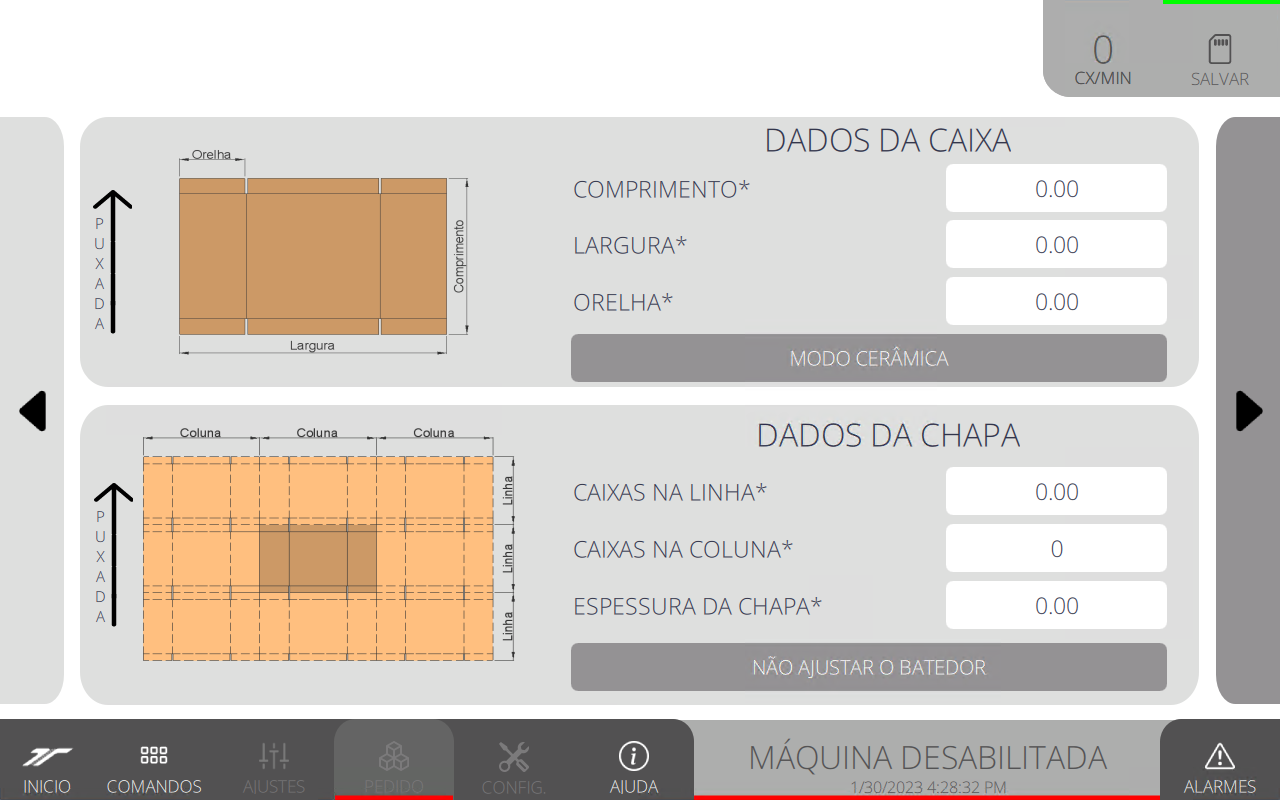
\includegraphics[width=480 px,height=300 px]{src/imagesICV/09-request/new/Tela-Principal-2.png}
\end{figure}
\vspace*{\fill}

\newpage
\thispagestyle{fancy}
\vspace*{40 pt}
\subsubsection{\small{Dados da caixa}} \label{sec:telaNovoPedidoP2DadosCaixa}
\vspace*{\fill}
\begin{figure}[h]
    \centering
    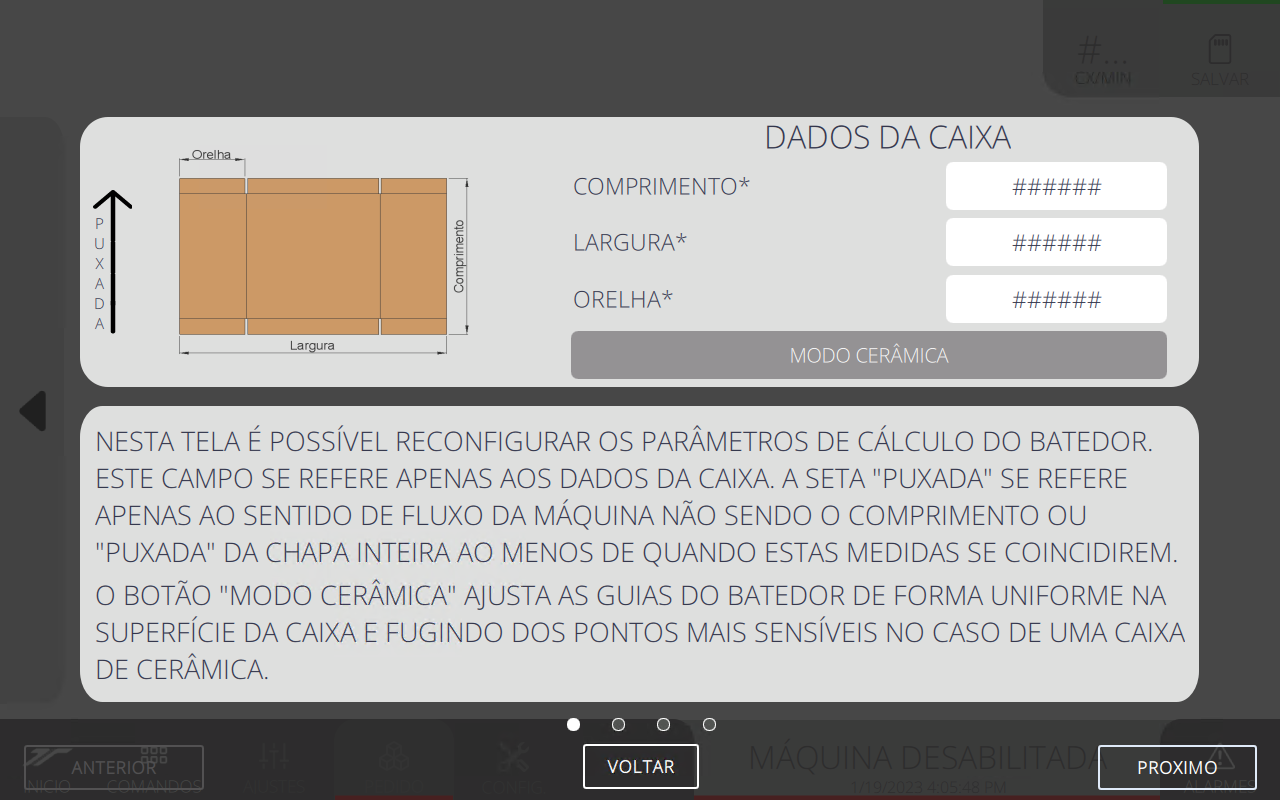
\includegraphics[width=576 px,height=360 px]{src/imagesICV/09-request/new/e-6.png}
\end{figure}
\vspace*{\fill}

\newpage
\thispagestyle{fancy}
\vspace*{40 pt}
\subsubsection{\small{Dados da Chapa}} \label{sec:telaNovoPedidoP2DadosChapa}
\vspace*{\fill}
\begin{figure}[h]
    \centering
    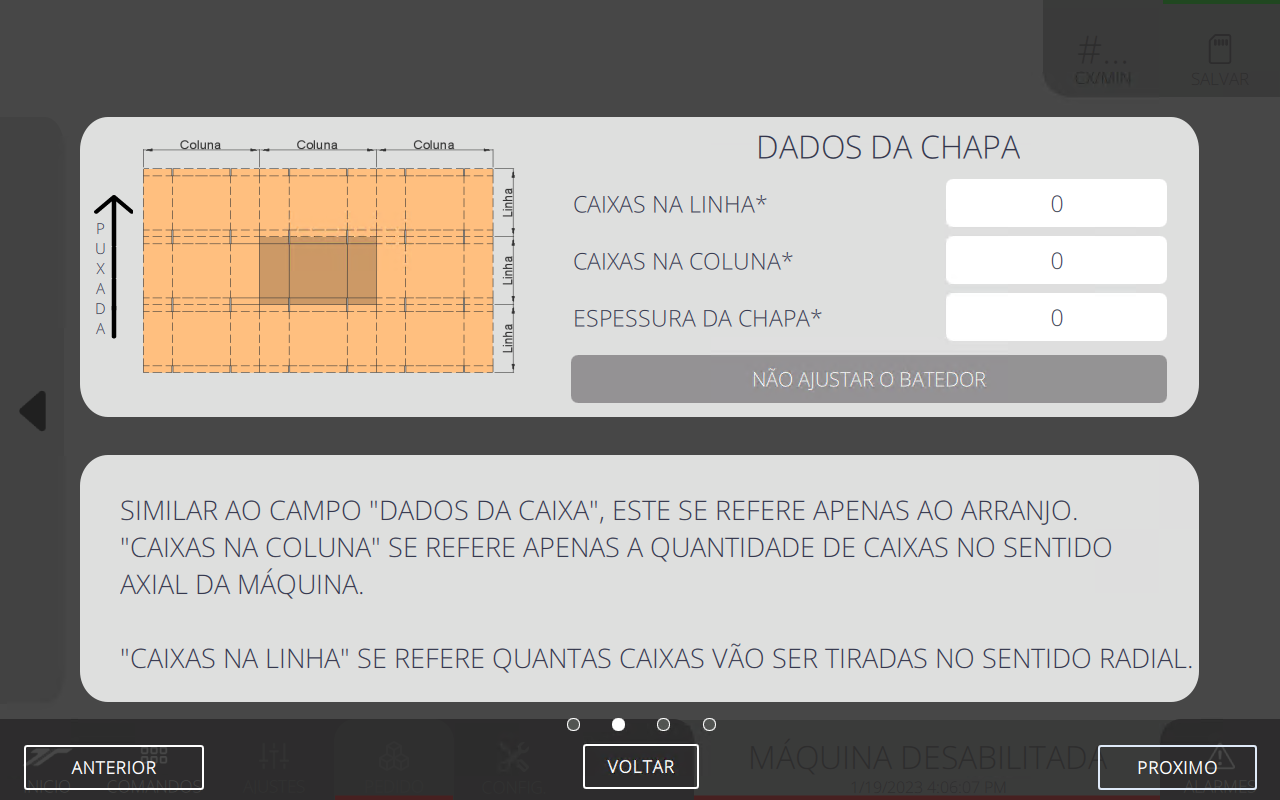
\includegraphics[width=576 px,height=360 px]{src/imagesICV/09-request/new/e-7.png}
\end{figure}
\vspace*{\fill}

\newpage
\thispagestyle{fancy}
\vspace*{40 pt}
\subsubsection{\small{Não ajustar batedor}} \label{sec:telaNovoPedidoP2NaoAjustarBatedor}
\vspace*{\fill}
\begin{figure}[h]
    \centering
    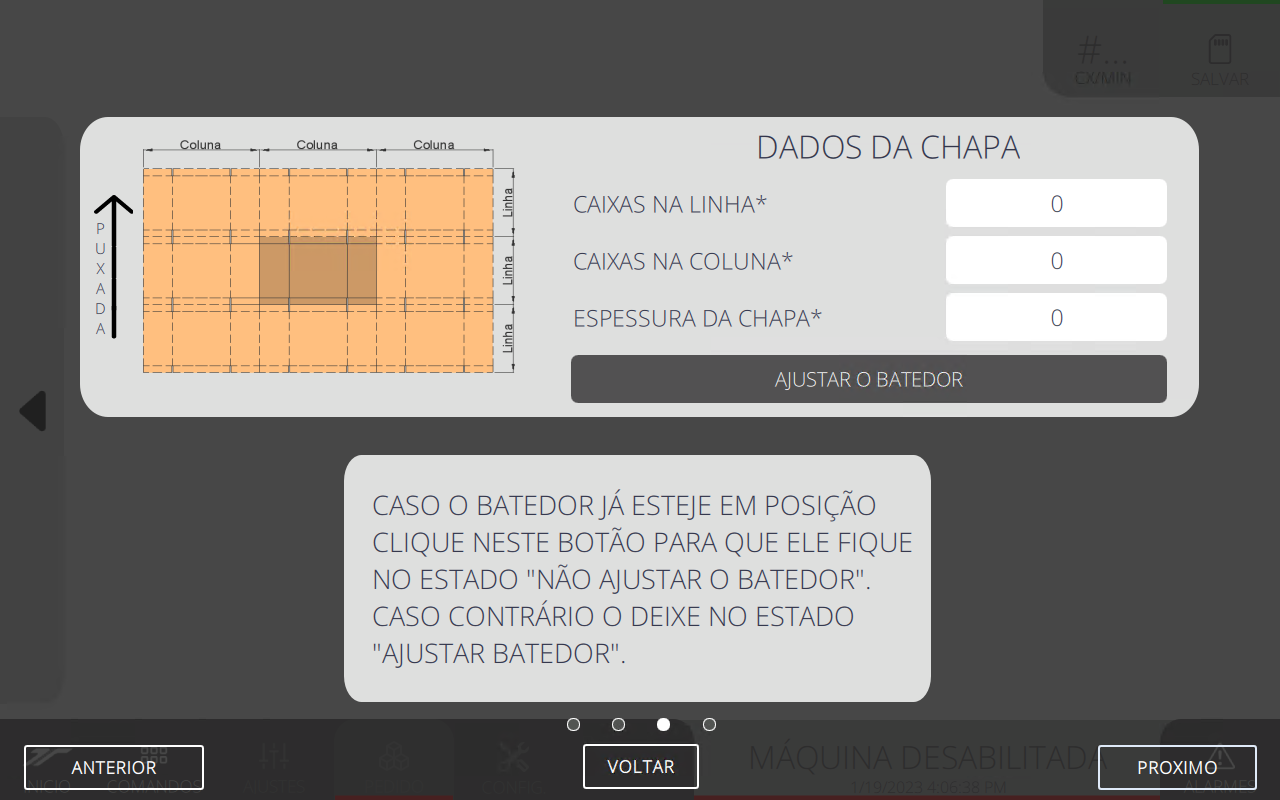
\includegraphics[width=576 px,height=360 px]{src/imagesICV/09-request/new/e-8-COM-ERRO-DIGITAÇÃO.png}
\end{figure}
\vspace*{\fill}

\newpage
\thispagestyle{fancy}
\vspace*{40 pt}
\subsubsection{\small{Requisitos para liberar a próxima página}} \label{sec:telaNovoPedidoP2RequisitosLiberarProximaPagina}
\vspace*{\fill}
\begin{figure}[h]
    \centering
    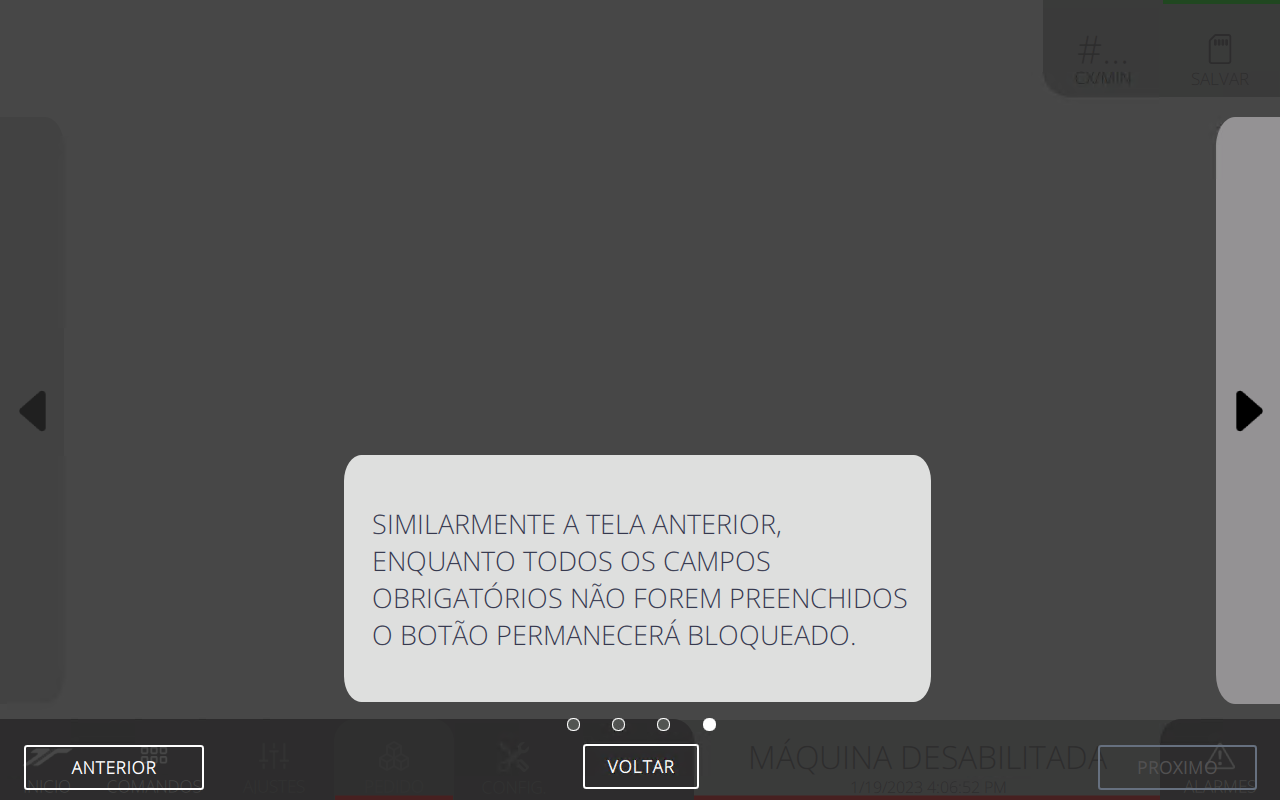
\includegraphics[width=576 px,height=360 px]{src/imagesICV/09-request/new/e-9.png}
\end{figure}
\vspace*{\fill}
